\documentclass[11pt]{article}
\usepackage[a4paper,margin=1.9cm]{geometry}
\usepackage{graphicx}
\usepackage{booktabs}
\usepackage{xcolor}
\usepackage{amsmath}
\usepackage{enumitem}
\usepackage[hidelinks]{hyperref}
\usepackage{titlesec}
\usepackage{caption}
\usepackage{tcolorbox}
\usepackage{float}

\captionsetup{font=small,labelfont=bf}
\setlist{nosep,leftmargin=1.3em}
\titlespacing*{\section}{0pt}{1.0ex}{0.5ex}
\titlespacing*{\subsection}{0pt}{0.7ex}{0.3ex}
\titleformat{\section}{\large\bfseries}{\thesection}{0.6em}{}
\titleformat{\subsection}{\normalsize\bfseries}{\thesubsection}{0.6em}{}
\setlength{\parskip}{0.35em}
\setlength{\parindent}{0pt}

\definecolor{accent}{HTML}{1f6feb}
\definecolor{kill}{HTML}{9e2a2b}
\newcommand{\code}[1]{\texttt{\small #1}}

\begin{document}

\begin{center}
 {\LARGE\bfseries The Alpha Factory}\\[2pt]
 {\large A miniature strategy factory and a validation gate}\\[4pt]
 {\normalsize Clarion Capital take-home $\cdot$ quantitative trader}\\[2pt]
 {\footnotesize Pre-registered criteria \code{config/gate\_criteria.yaml} $\cdot$
  SHA-256 \code{8e35cb92eb5f\ldots d5d8eab} (thresholds unchanged across all strategy iterations; one documented L2 redesign)}
\end{center}

\begin{tcolorbox}[colback=kill!5,colframe=kill!70,boxrule=0.6pt,arc=2pt,
 left=6pt,right=6pt,top=4pt,bottom=4pt]
\textbf{Verdict, 48 candidates in, 0 survivors out.}
The factory builds 48 instances from two opposed root ideas, a volatility-targeted
trend follower and a filtered mean-reversion, across four markets. Run as four
\emph{independent} layers on the full population, the gate clears no instance through
all four. The strongest candidate (the vol-targeted trend on ETH, one of only
three instances to clear both the out-of-sample and walk-forward layers, full-sample
Sharpe $1.17$, individually significant at permutation $p=0.001$) still fails: it
breaches the drawdown cap in the COVID crash, and its \textbf{Deflated Sharpe Ratio
is $0.35$}, far below the $0.95$ gate. \emph{Nothing here is alpha.}
\end{tcolorbox}

\section{Two opposed root ideas}
The factory ships two families that bet on \emph{opposite} market hypotheses, so a
population that ``works'' cannot be one bet wearing two hats. Each exposes
\textbf{at most two free parameters}; every other choice is fixed by design, so the
optimiser has almost no surface to overfit.

\begin{itemize}
\item \textbf{\code{voltarget\_mom}, vol-targeted momentum (trend).} The
sign of the \code{lookback}-bar return, with the position scaled by (trailing
typical volatility / current \code{vol\_win} volatility): larger in calm, smaller in
turbulence. Volatility targeting is the most replicated way to improve a trend
signal's risk-adjusted return. The normalising horizon and a leverage cap are fixed;
the position is a continuous risk-scaled exposure, which the backtester sizes
natively. \emph{Free:} \code{lookback}, \code{vol\_win}.
\item \textbf{\code{bollinger\_revert}, filtered mean reversion (reversal).} Fade
a deviation of $k$ standard deviations from the \code{n}-bar mean, \emph{take profit
when price crosses back through that mean}, and stay flat between trades. A fixed
longer-horizon $z$-score gates entries, we do \emph{not} fade while a strong trend
is underway, the classic way naive reversion dies. \emph{Free:} \code{n}, \code{k}.
\end{itemize}

One bets that moves continue; the other bets that stretched moves revert. Both
include an explicit exit and a regime control, so neither is a toy. Architecturally a
family is one subclass with a \code{signal()} method and a parameter grid, registered
through \code{families.register()}; \textbf{adding a third root idea is a single
\code{register()} call} and the factory, backtester, gate, figures and report pick it
up with no other change, the extensibility the brief asks for.

\textbf{Which two parameters are free is deliberate.} For the trend, \code{lookback}
(the momentum horizon) and \code{vol\_win} (how responsive the volatility estimate is)
are freed because neither has a canonical correct value and both directly express the
hypothesis; the normalising volatility horizon (a $\sim$3-month baseline, a reference
scale) and the leverage cap (a risk limit) are fixed, since optimising a baseline, or
letting the backtest raise leverage to chase return, is a textbook overfit. The
reversion family is symmetric: \code{n} (the timescale of a stretched move) and
\code{k} (how many sigmas to fade) are the genuine knobs, while the trend-strength
gate (a regime filter) and the mean-cross exit (the definitional close of the trade)
are fixed by design rather than tuned.

\textbf{Population.} Each family has a 6-point grid, expanded across four
markets, the S\&P~500 index (SPXUSD), USD/JPY, gold (XAUUSD) and ETH/USD. That is
$2\times6\times4=\mathbf{48}$ instances.

\begin{figure}[h]\centering
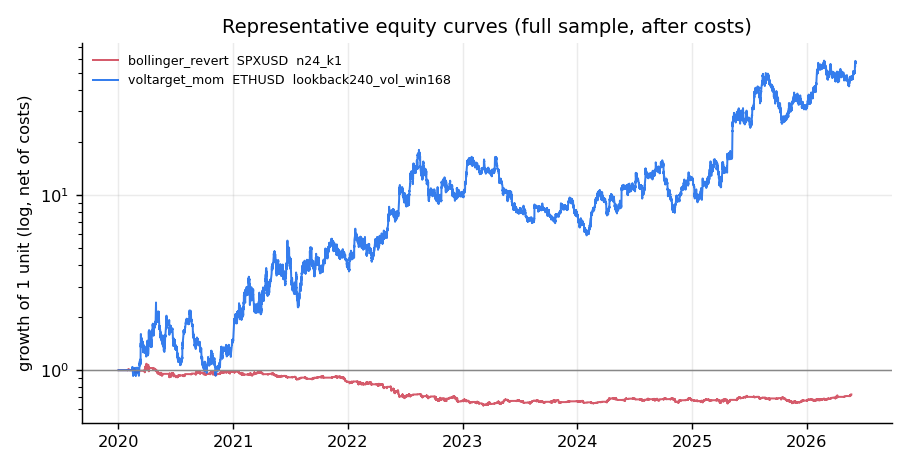
\includegraphics[width=0.86\linewidth]{figures/equity_curves.png}
\caption{The best instance of each family by out-of-sample Sharpe, net of costs, on a
log scale. The vol-targeted trend (blue) is the strongest the factory produced; the
best reversion instance (red) barely breaks even net of costs. Both are rejected by
the full gate.}
\label{fig:equity}
\end{figure}

\section{Realism: data, costs, no look-ahead}
\textbf{Data.} The four supplied MetaTrader M1 CSVs (Jan~2020 -- mid~2026,
$\sim$2.4M rows each) are resampled to \textbf{H1}. Hours with no ticks are
\emph{dropped, not forward-filled}, preserving genuine gap risk. After cleaning each
series carries 38k--40k bars ($\sim$6{,}100 bars/year).

\textbf{No look-ahead.} Signals use only information up to each bar's close, and the
backtester applies a strict \textbf{one-bar execution lag}: the position over
bar~$t$ is the signal from bar~$t-1$. An explicit test confirms that truncating
future data leaves every past signal bit-identical for both families.

\textbf{Costs.} The pre-registered model is the brief's default: the realised
half-spread from \code{<SPREAD>} on each side of a position change, plus
$0.5$\,bps/side commission on turnover. Measured mean spreads track the asset
hierarchy: USD/JPY $0.57$\,bps, SPXUSD $0.69$\,bps, XAUUSD $1.11$\,bps, ETHUSD
$8.18$\,bps. Costs are what most candidates die against, and the two families fail for opposite
reasons (Figure~\ref{fig:costs}). The reversion grid is in fact the \emph{lower}-turnover
family (it stays flat between trades) and loses even \emph{gross}: its problem is a weak
signal, with costs only a secondary nail. The vol-targeted trend is the
\emph{higher}-turnover family (it re-scales every bar) and is where costs bite hardest,
eroding a genuine gross edge, on USD/JPY and gold turning a positive gross Sharpe into
break-even or loss.

\begin{figure}[H]\centering
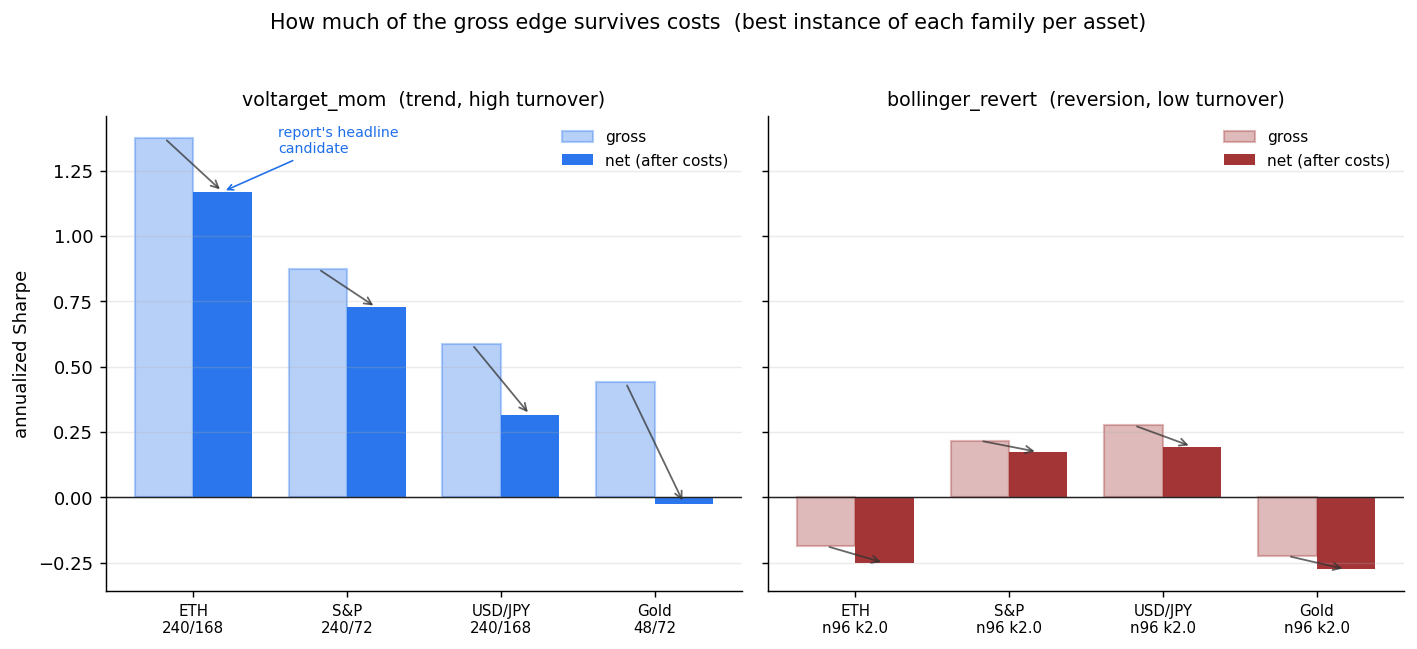
\includegraphics[width=0.95\linewidth]{figures/cost_drag.png}
\caption{How much of the gross edge survives trading costs: gross vs.\ net annualised
Sharpe for the best instance of each family on each asset (parameters labelled). The
trend family (left) has a real gross edge that its high turnover erodes, wiping it out
on USD/JPY and gold; the reversion family (right) turns over little, so costs barely
bite, but its signal is weak even gross.}
\label{fig:costs}
\end{figure}

\section{Pre-registered pass/fail criteria and honesty}
Every threshold is fixed in \code{config/gate\_criteria.yaml} \emph{before} the gate
runs; \code{run.py} prints its SHA-256, which is \textbf{identical across every
strategy iteration} of this project. The strategies changed; the gate never did. The
full timeline is in \code{DECISIONS.md}.

\begin{center}\small
\begin{tabular}{@{}lll@{}}
\toprule
\textbf{Layer} & \textbf{Test} & \textbf{Pre-registered pass condition} \\
\midrule
L1 & IS/OoS + robustness & OoS Sharpe $\ge 0.50$, OoS return $>0$, and every \\
  &           & $\pm20\%$ neighbour Sharpe $\ge 0$ (median $\ge 0.30$) \\
L2 & Walk-forward    & per instance (fixed params): aggregated out-of- \\
  & (rolling windows)  & window Sharpe $\ge 0.50$ and positive in $\ge 60\%$ of windows \\
L3 & Stress replay    & over COVID + the instance's own 2 worst 21-day windows: \\
  &           & return $\ge -10\%$, DD $\le 20\%$; Sharpe $\ge 0$ under vol-only $2\times$ \\
L4 & Monte Carlo + DSR  & block-permutation $p<0.05$ and DSR $\ge 0.95$ ($N{=}48$) \\
\bottomrule
\end{tabular}
\end{center}

Each layer is run \textbf{independently on all 48 instances}; the funnel is the
\emph{intersection} of the four verdicts, not a sequential filter that hides what the
later layers would reject.

\section{The four-layer gate, what each layer found}

\subsection{L1, in-sample / out-of-sample + parameter robustness}
First 70\% in-sample, last 30\% out-of-sample; an instance passes only if its OoS
performance clears the bar \emph{and} a $\pm20\%$ perturbation of each parameter
leaves no losing neighbour. Because the parameters are \emph{fixed}, the in-sample
slice trains nothing, so this is a soft recent-holdout rather than a fit-then-validate
step; L1's real anti-overfitting teeth is the $\pm20\%$ robustness, while the main
overfitting source (selecting among 48 designer-chosen configs) is paid for by L2 and,
above all, the Deflated Sharpe. \textbf{Result: 4/48 pass} (Figure~\ref{fig:oos}), all
vol-targeted trends on ETH (OoS Sharpe up to $1.52$). The reversion family clears
none: faded short-horizon deviations do not survive out-of-sample net of costs. The
full parameter landscape (Figure~\ref{fig:surface}) shows the strong region is a
broad \emph{plateau} rather than a lone spike, which is exactly what the $\pm20\%$
robustness check formalises.

\begin{figure}[H]\centering
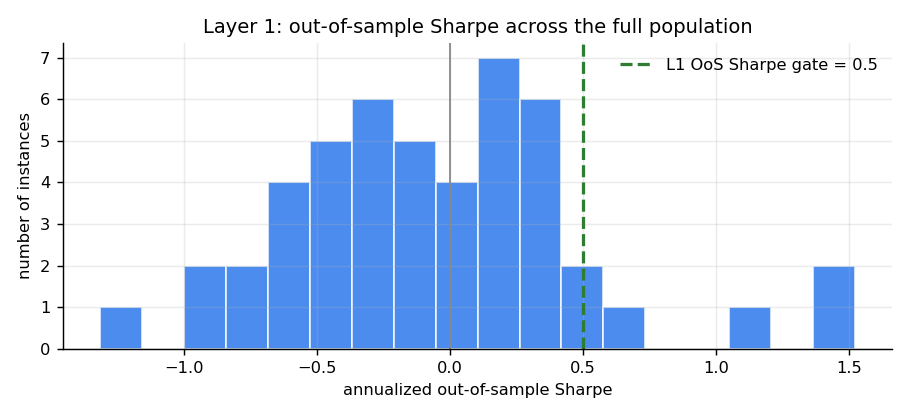
\includegraphics[width=0.86\linewidth]{figures/oos_sharpe.png}
\caption{Layer 1: distribution of annualised out-of-sample Sharpe across all 48
instances. Only a thin right tail (vol-targeted trends on ETH) clears the $0.50$
gate; the bulk sit at or below zero out-of-sample.}
\label{fig:oos}
\end{figure}

\begin{figure}[h]\centering
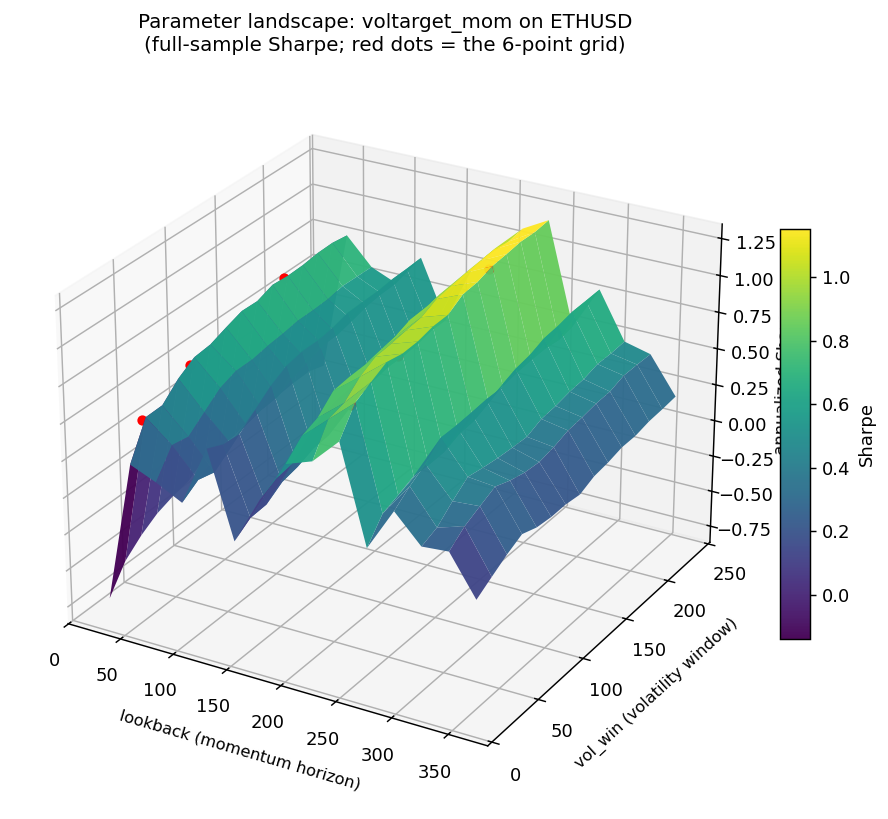
\includegraphics[width=0.74\linewidth]{figures/param_surface_eth.png}
\caption{The parameter landscape behind L1's robustness check: full-sample Sharpe of
\code{voltarget\_mom} on ETH over a dense \code{lookback}$\times$\code{vol\_win} mesh
(red dots mark the six pre-registered grid points). This is a \emph{diagnostic}, a
dense scan visualised here, adding nothing to the $N=48$ trial count. The profitable
region is a broad plateau, not a narrow peak: a Sharpe perched on a spike would be
overfit and would fail the $\pm20\%$ neighbour test.}
\label{fig:surface}
\end{figure}

\subsection{L2, walk-forward stability (per instance)}
With the instance's \emph{fixed} parameters (so nothing is trained), step a 30-week
test window through the series (after an initial 90-week span) and judge the instance on
its own out-of-window record: aggregated Sharpe $\ge0.50$ \emph{and} a positive return in
$\ge60\%$ of windows. This verdict is
independent per instance, the temporal-stability complement to L1's single split
(a strategy can pass one and fail the other). \textbf{Result: 6/48 pass}, all
vol-targeted trends with the long ($240$-bar) horizon, on ETH and the S\&P. A rolling
\emph{re-optimisation} (one curve per family/market, plus each instance's
parameter-selection frequency) is computed as a \emph{diagnostic} only: an earlier
design that gated on the selection frequency was relative across the grid, its
pass count was capped by grid arithmetic and a strong stand-alone instance could
fail for being the runner-up, so it was demoted (see \code{DECISIONS.md}).

\subsection{L3, stress replay (real + synthetic)}
A fixed COVID window plus the two worst rolling 21-day windows \emph{of each
instance's own equity}, a momentum book can be short in a crash and profit, so its
true worst case is a sharp reversal a market-drawdown window would miss, and a
\emph{volatility-only} $2\times$ synthetic path (only the deviations are scaled, the
drift held, so it does not flatter trend). ``Acceptable'' (return $\ge-10\%$, DD
$\le20\%$, synthetic Sharpe $\ge0$) was fixed in advance. \textbf{Result: 8/48
pass}, all on USD/JPY, the calmest market. The dominant kill is the COVID window; the
own-worst-window test also exposes a $47\%$ drawdown in the ETH trend's worst 21 days,
and L3 removes the three instances that had cleared both L1 and L2.

\subsection{L4, Monte Carlo + Deflated Sharpe Ratio}
A \emph{block}-permutation test against a no-skill null, shuffling the order of
$\sim$1-day return blocks, so the null keeps the volatility clustering an i.i.d.
shuffle would erase, a moving-block bootstrap (block $=24$ bars) for the drawdown
distribution (a \emph{diagnostic}, not gated), and the Deflated Sharpe Ratio with
\code{n\_trials} set to the \emph{total number of instances, $N=48$}. The permutation only
asks whether the edge is real on \emph{this} series; paying for having tried 48 of them is
the Deflated Sharpe's job.
\textbf{Result: 0/48 pass}, the subject of \S6.

\section{Survival funnel}
\begin{figure}[h]\centering
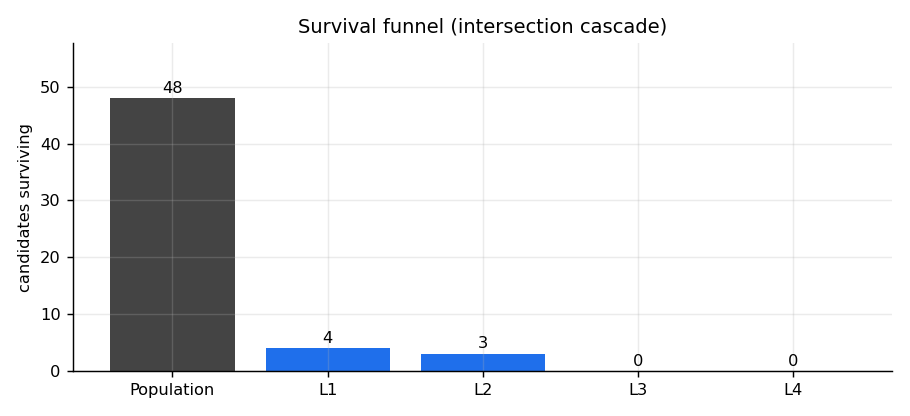
\includegraphics[width=0.92\linewidth]{figures/funnel.png}
\caption{Intersection cascade. L1 admits 4 instances; three of them also clear the
walk-forward stability test (L2), and the COVID stress window (L3) then removes all
three. The intersection of all four layers is empty.}
\label{fig:funnel}
\end{figure}

\begin{center}\small
\textbf{Per-layer view (each layer judged independently on all 48)}\\[2pt]
\begin{tabular}{@{}llccl@{}}
\toprule
Layer & Test & Pass & Fail & Dominant failure reason \\
\midrule
L1 & IS/OoS + robustness    & 4 & 44 & OoS Sharpe below threshold \\
L2 & Walk-forward        & 6 & 42 & out-of-window Sharpe/return below bar \\
L3 & Stress replay       & 8 & 40 & blows up in COVID window \\
L4 & Monte Carlo + DSR     & 0 & 48 & no skill (permutation) \emph{and} fails DSR \\
\midrule
\multicolumn{2}{@{}l}{\textbf{Intersection (all four)}} & \textbf{0} & \textbf{48} & --- \\
\bottomrule
\end{tabular}
\end{center}

Three instances clear both L1 and L2 (the long-horizon ETH vol-targeted trends), and
no instance clears three layers: a holdout split and a rolling-stability test agree
only on a handful of trend instances, and none of those survives the COVID crisis.

\section{The Deflated Sharpe verdict}
This is the heart of the exercise. We did not test one strategy; we tested 48. The
expected maximum Sharpe of $N=48$ zero-skill trials is, on this data, a
per-observation $\text{SR}^\star\approx0.0168$, an \textbf{annualised hurdle near
$1.3$} that a strategy must clear before its Sharpe is even evidence of skill.

\begin{figure}[h]\centering
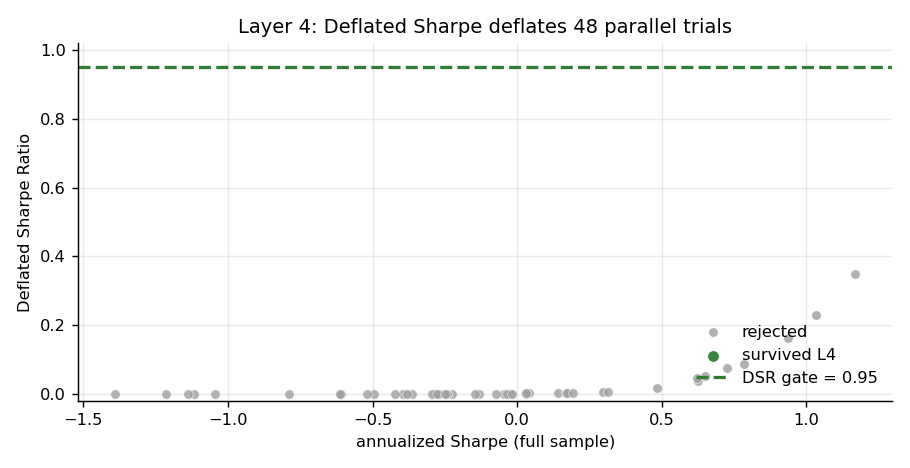
\includegraphics[width=0.92\linewidth]{figures/dsr_scatter.png}
\caption{Deflated Sharpe vs.\ raw annualised Sharpe across all 48 instances. The best
DSR is $0.35$ (the ETH vol-targeted trend, raw Sharpe $1.17$); the $0.95$ gate is
never reached. Higher raw Sharpe buys very little once 48 parallel trials are
deflated.}
\label{fig:dsr}
\end{figure}

The sharpest illustration is the best candidate itself. The ETH vol-targeted trend
is one of three instances to pass both L1 and L2, with a full-sample Sharpe of $1.17$, a
permutation $p=0.001$, and positive returns in most bootstrap resamples. Judged alone
it looks real. Judged honestly, as one of $48$ things we tried, and against the
COVID crash, it is rejected twice over: its Deflated Sharpe is $0.35$, and it
breaches the $20\%$ drawdown cap in 2020. The multiple-testing correction is not a
footnote; it is the verdict, and it is why ``just generate more candidates'' cannot
manufacture a survivor, every instance added only raises the bar
(\code{n\_trials}) for all of them. The flip side is that the Deflated Sharpe depends on
the \emph{declared} trial count: a Sharpe earned by one pre-committed hypothesis is
genuinely stronger evidence than the same number cherry-picked as the best of 48, so the
only way to flatter it is to \emph{under-report} $N$, which is dishonesty rather than
method and is auditable here from the code that builds all 48. The principled adjustment
runs the other way, through the effective trial count below.

\section{Verdict, limitations, and honesty}
\textbf{Verdict: deploy nothing.} On this data with these (pre-registered, demanding)
criteria, $48\rightarrow0$ is the right answer. The factory manufactured plausible
candidates, including one genuinely convincing in isolation, and the gate
refused to be impressed by any of them.

\textbf{What would change the verdict.} A deployable instance would have to clear OoS
\emph{and} walk-forward (L1$\cap$L2), hold its floor through COVID and a $2\times$-vol
path (L3), and post a Deflated Sharpe $\ge0.95$, which at $N=48$ demands an
annualised, stress-robust Sharpe well above the $1.17$ the best candidate reached.

\textbf{Honesty.} The strategies were iterated during development (a dual-SMA/z-score
pair, then a multi-timeframe momentum/breakout pair, a vol-targeting family added to
demonstrate extensibility, and finally the two opposed families here); across all
four iterations the \code{gate\_criteria.yaml} SHA-256 was \emph{identical}, the
proof that no threshold was ever tuned to admit a candidate. The config then changed
once, deliberately, when L2's \emph{methodology} was redesigned: its original verdict
re-optimised the grid and judged each instance \emph{relative} to its siblings
(capped by grid arithmetic, decided by a noisy in-sample ranking), so a strong
stand-alone instance could fail merely for being the runner-up. L2 is now an
\emph{independent} per-instance stability test (fixed parameters, consistency across
rolling out-of-window windows), with the re-optimisation retained as a diagnostic.
The change is documented, raised L2's pass count from $1$ to $6$, and \emph{left the
verdict unchanged} ($48\rightarrow0$), confirming it fixed a design flaw rather
than admitting anything. Two further methodology refinements touched no threshold (the SHA-256 is unchanged):
L3 now stresses each instance over its \emph{own} worst 21-day windows (a market-drawdown
window misses a strategy whose worst case is a sharp reversal) and uses a volatility-only
synthetic shock (doubling volatility without flattering trend), and L4's significance test
is now a block permutation that preserves serial structure (an i.i.d.\ shuffle was
anti-conservative). Both left the verdict unchanged.
\code{DECISIONS.md} records the full timeline.

\textbf{Correlated trials and effective \emph{N}.} The Deflated Sharpe uses the raw
trial count $N=48$, but the 48 instances are not independent: within each
family/market the six grid points are correlated (mean pairwise correlation
$\approx0.60$), while the two opposed families are \emph{negatively} correlated
($\approx-0.30$, which validates the design). A participation-ratio count of the
$48\times48$ correlation matrix gives an effective $N\approx12$, not 48. Using
$N\approx12$ raises the best instance's Deflated Sharpe from $0.35$ to $0.69$ ---
still well below the $0.95$ gate. We report the conservative raw $N=48$; the verdict
is unchanged under either count, and an effective-$N$ deflation is the natural
refinement for a future iteration.

\textbf{Limitations.} Two families and coarse grids; a single timeframe (H1); a cost
model using mean bar spread without slippage/impact; and the DSR's raw (rather than
effective) trial count, kept deliberately as the conservative choice. Each is a
deliberate simplicity trade and a candidate next iteration, a richer factory,
never a looser gate.

\end{document}
